\newpage
\clearpage
\section{Detector setup}
    \subsection{Large Hadron Collider}
        The Large Hadron Collider (LHC) is the world's largest circular accelerator. Figure \ref{LHC} shows that the LHC and its major experimental groups are located near Geneva, Switzerland. LHC Run 1 was conducted from 2009 to 2013, and Run 2 occurred from 2015 to 2018.\@ The ongoing Run 3 is scheduled to collect physics data from 2022 to the summer of 2026.\@ During the run, most periods involve proton-proton collision measurements, with heavy-ion collision measurements conducted for about one month each year. The LHC accelerator hosts four major experimental groups: ATLAS, CMS, LHCb, and ALICE.\@
        \begin{figure}[htbp]
            \centering
            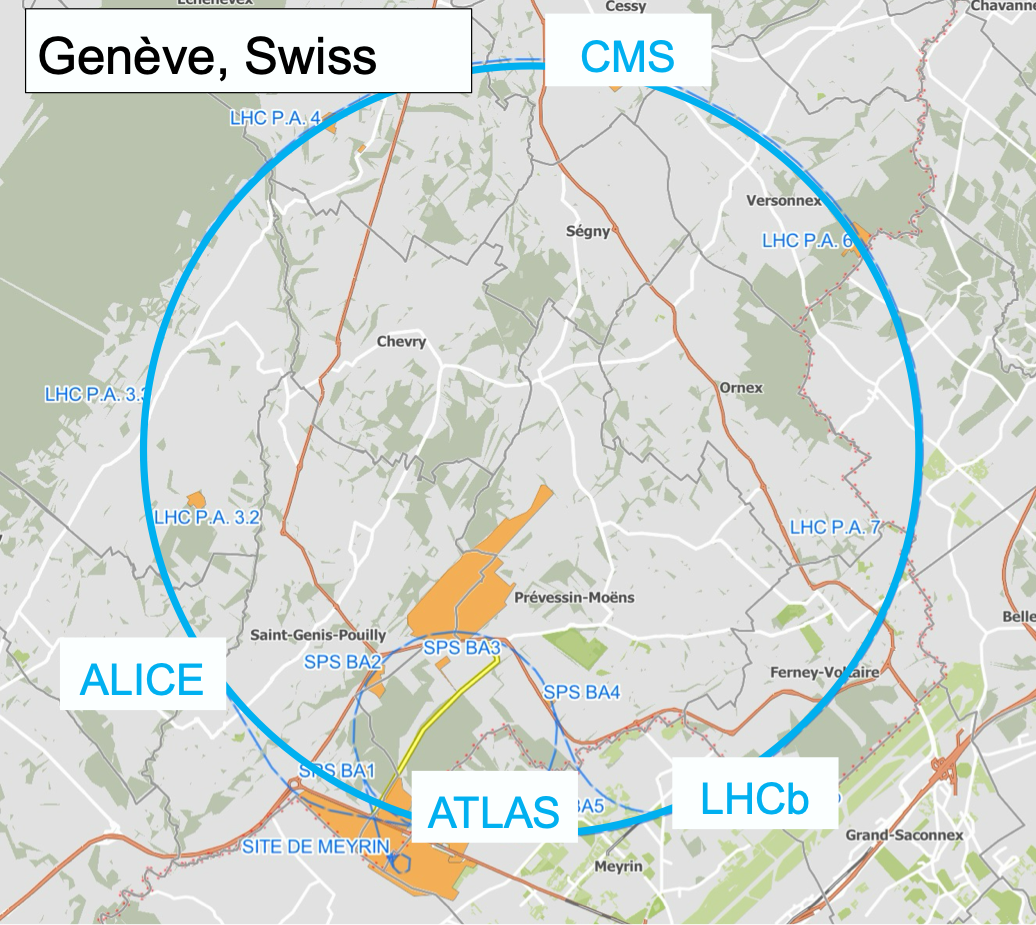
\includegraphics[keepaspectratio, scale=0.2]{fig/2_1_LHC_detecter.png}
            \caption{LHC}
            \label{LHC}
        \end{figure}
        \subsection{A Large Ion Collider Experiment}
        The A Large Ion Collider Experiment (ALICE) collaboration is an international collaboration of 168 research institutions from 40 countries and around 2,000 researchers. The overall view of the ALICE detector is shown in Figure \ref{ALICE_detectors}. The ALICE detector system is dedicated to research the Quark-Gluon Plasma (QGP) produced in heavy-ion collisions.
        \begin{figure}[htbp]
            \centering
            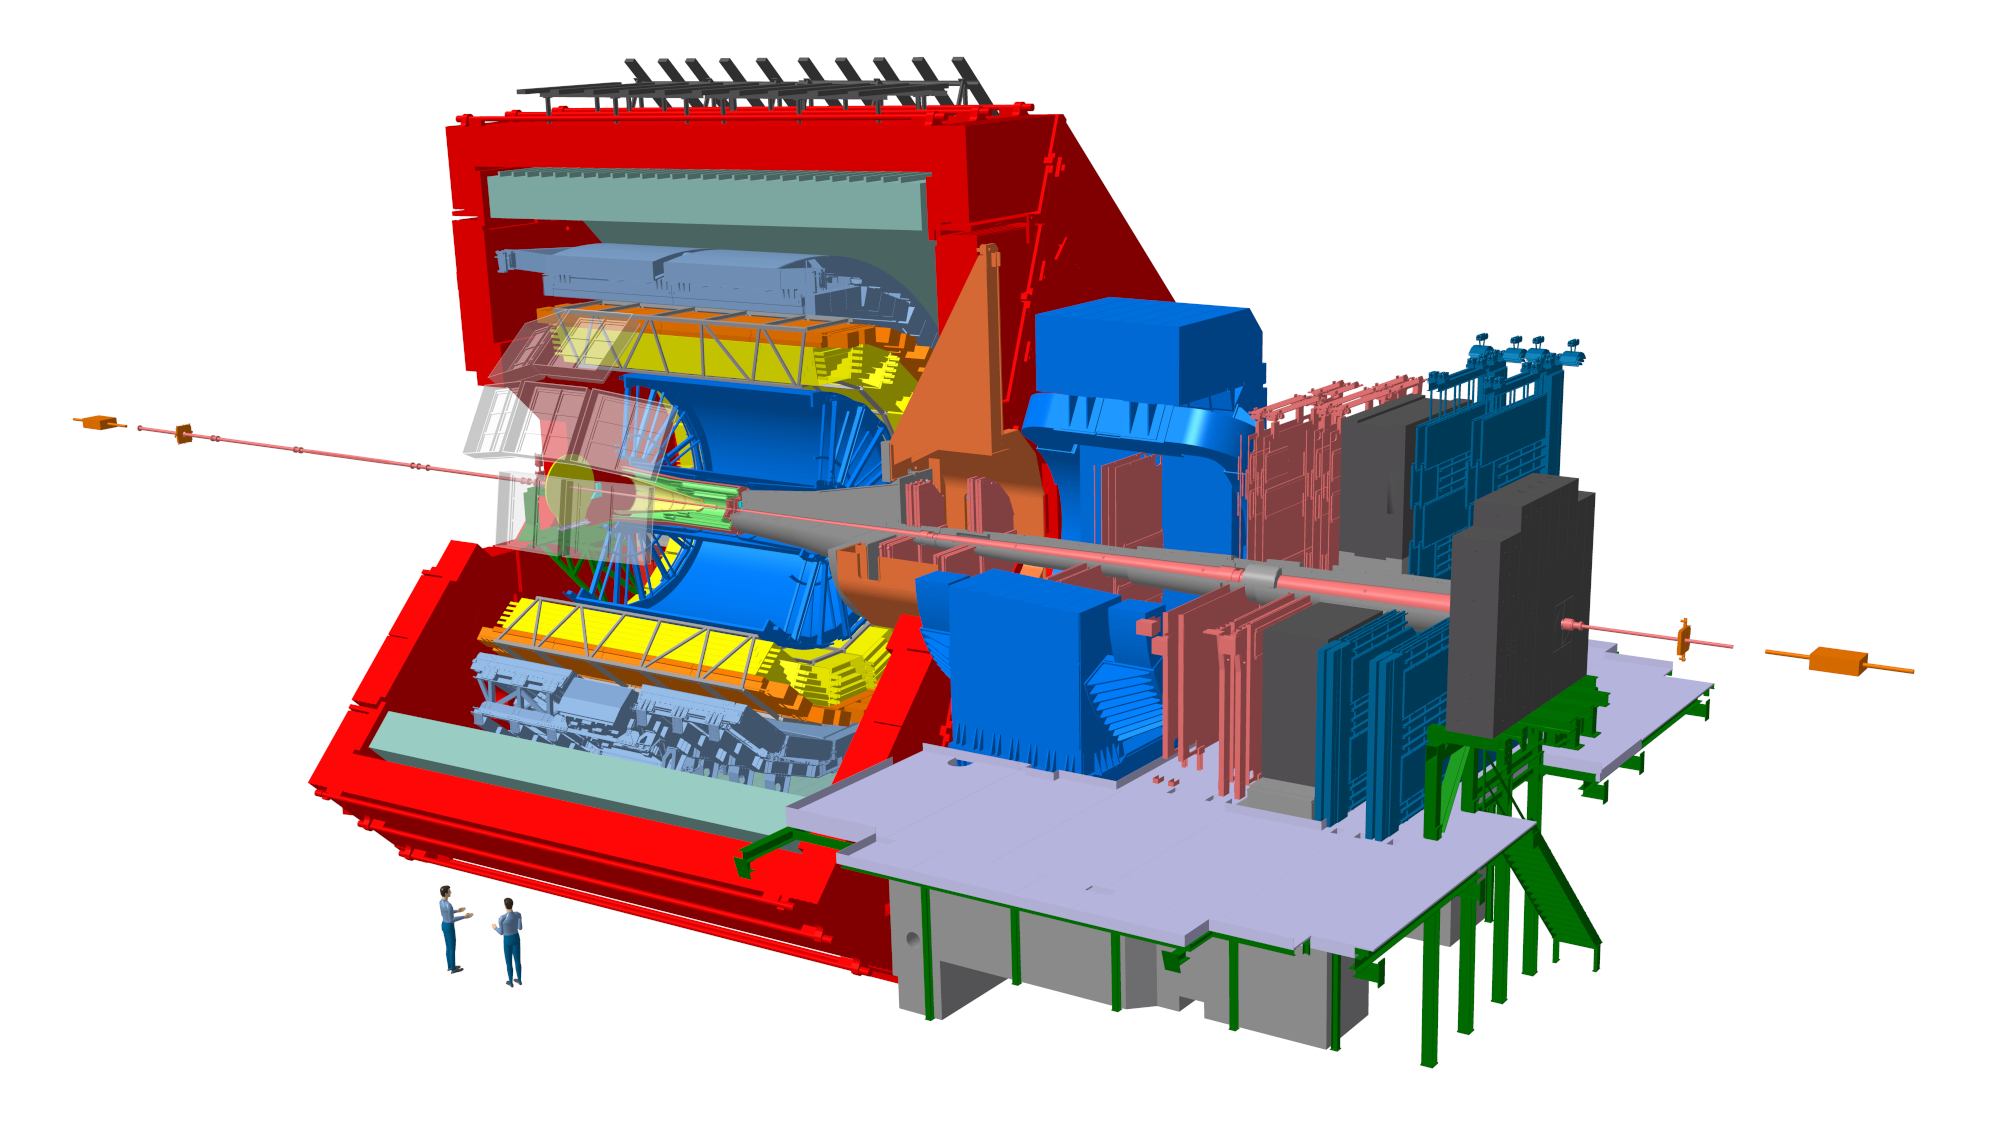
\includegraphics[keepaspectratio, scale=0.2]{fig/2_1_ALICE_RUN3_detectors.jpg}
            \caption{ALICE detectors}
            \label{ALICE_detectors}
        \end{figure}
        The detectors can be broadly divided into two main groups: the barrel detector and the forward detector.
        The barrel detector group includes ITS, TPC, TOF, EMCal, TRD, PHOS/CPV, and HMPID detectors.\@ A magnetic field is applied along the beam axis, bending the motion of charged particles and enabling particle identification, momentum, and energy measurements. The forward detector group is specifically designed for muon measurements and consists of three trackers—MFT, MCH, and MID—and two hadron absorbers. A dipole magnet is placed between MCH, allowing the measurement of muon momentum and sign. Other detectors include ZDC and FIT.\@ The ZDC is placed far from the collision point and measures the number of neutrons and protons, determining the centrality of heavy-ion collision events. The FIT detectors are placed forward and backwards near the collision point to measure the event luminosity and particle multiplicity.
        \subsubsection{MUON Spectrometer}
            \begin{figure}
                \centering
                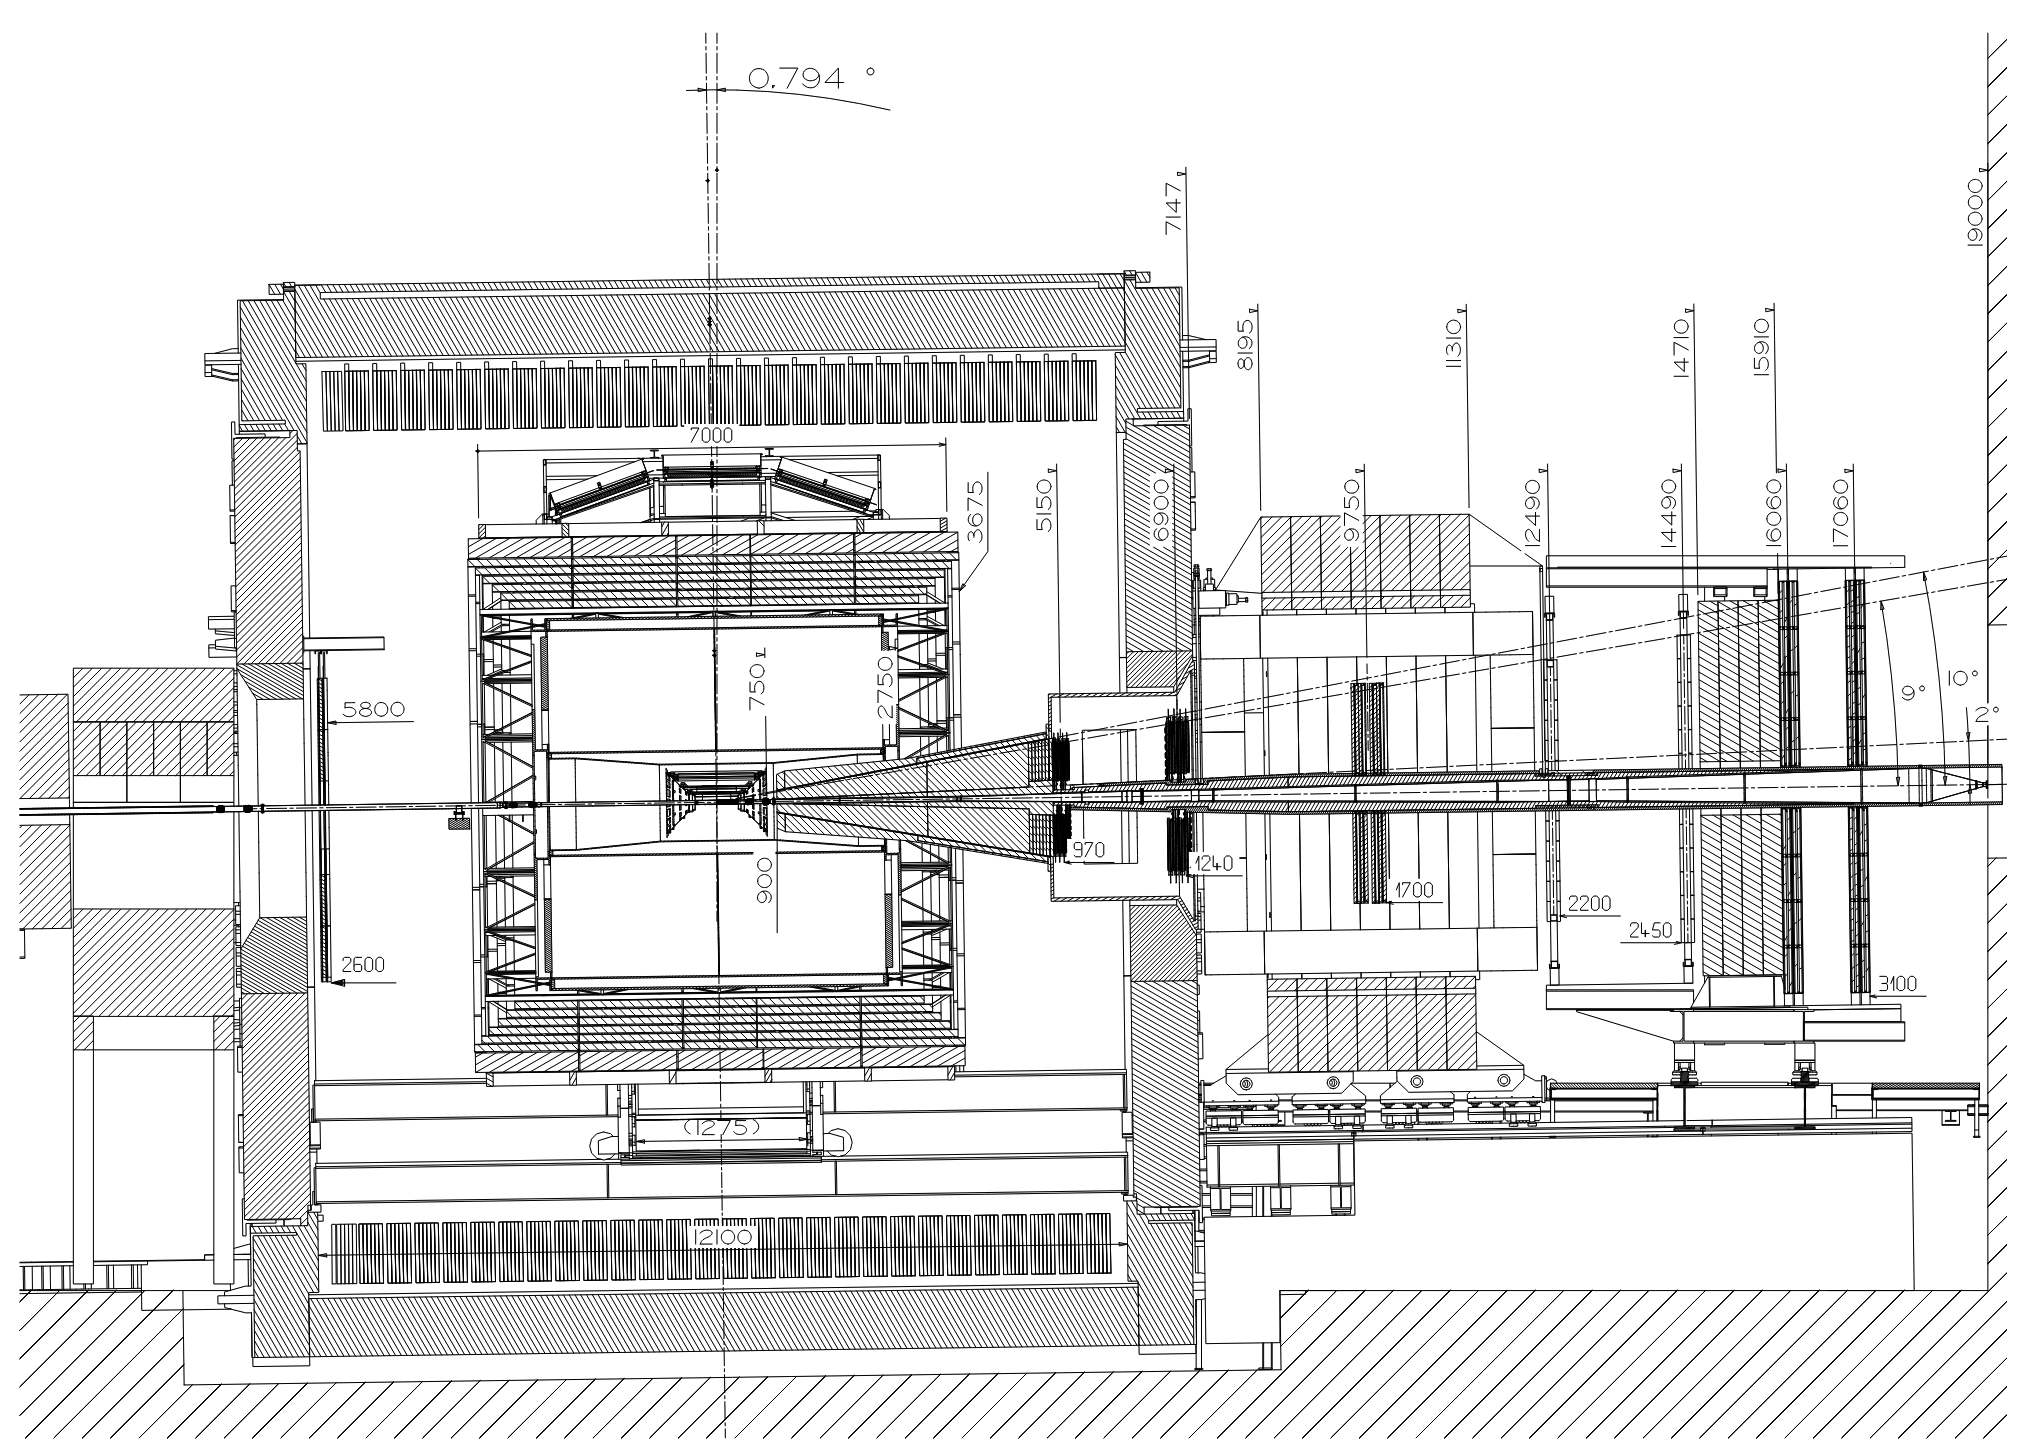
\includegraphics[keepaspectratio, scale=0.25]{fig/2_2_MUONspectrometer.png}
                \caption{MUON spectrometer}
                \label{MUONspectrometer}
            \end{figure}
            The MUON spectrometer is shown in Figure \ref{MUONspectrometer}\cite{Muon_TDR}.The MUON spectrometer consists of the Front Absorber, MCH, Iron Wall, and MID and has an acceptance range of $-4.0 < \eta < -2.5$. It uses the high penetration power of muons to identify them. Various particles generated at the collision point (IP) pass through the Front Absorber. Hadrons and light electrons, which interact strongly, are absorbed by the Front Absorber. The muons pass through it due to their high penetration power. The muons that pass through the Front Absorber are detected, and any particles such as $\pi$ mesons produced from interactions within the Front Absorber are measured by the MCH.\@ These particles are absorbed in the Iron Wall, so the MID does not detect them.\@ Therefore, muon identification is performed by combining tracks measured in the MCH and MID.\@ The momentum of the muons is measured using a dipole magnet in the MCH, which is set at a magnetic flux density of 3.0 $T/m^2$.\@
        \subsubsection{MFT}
            \begin{figure}[htbp]
                \centering
                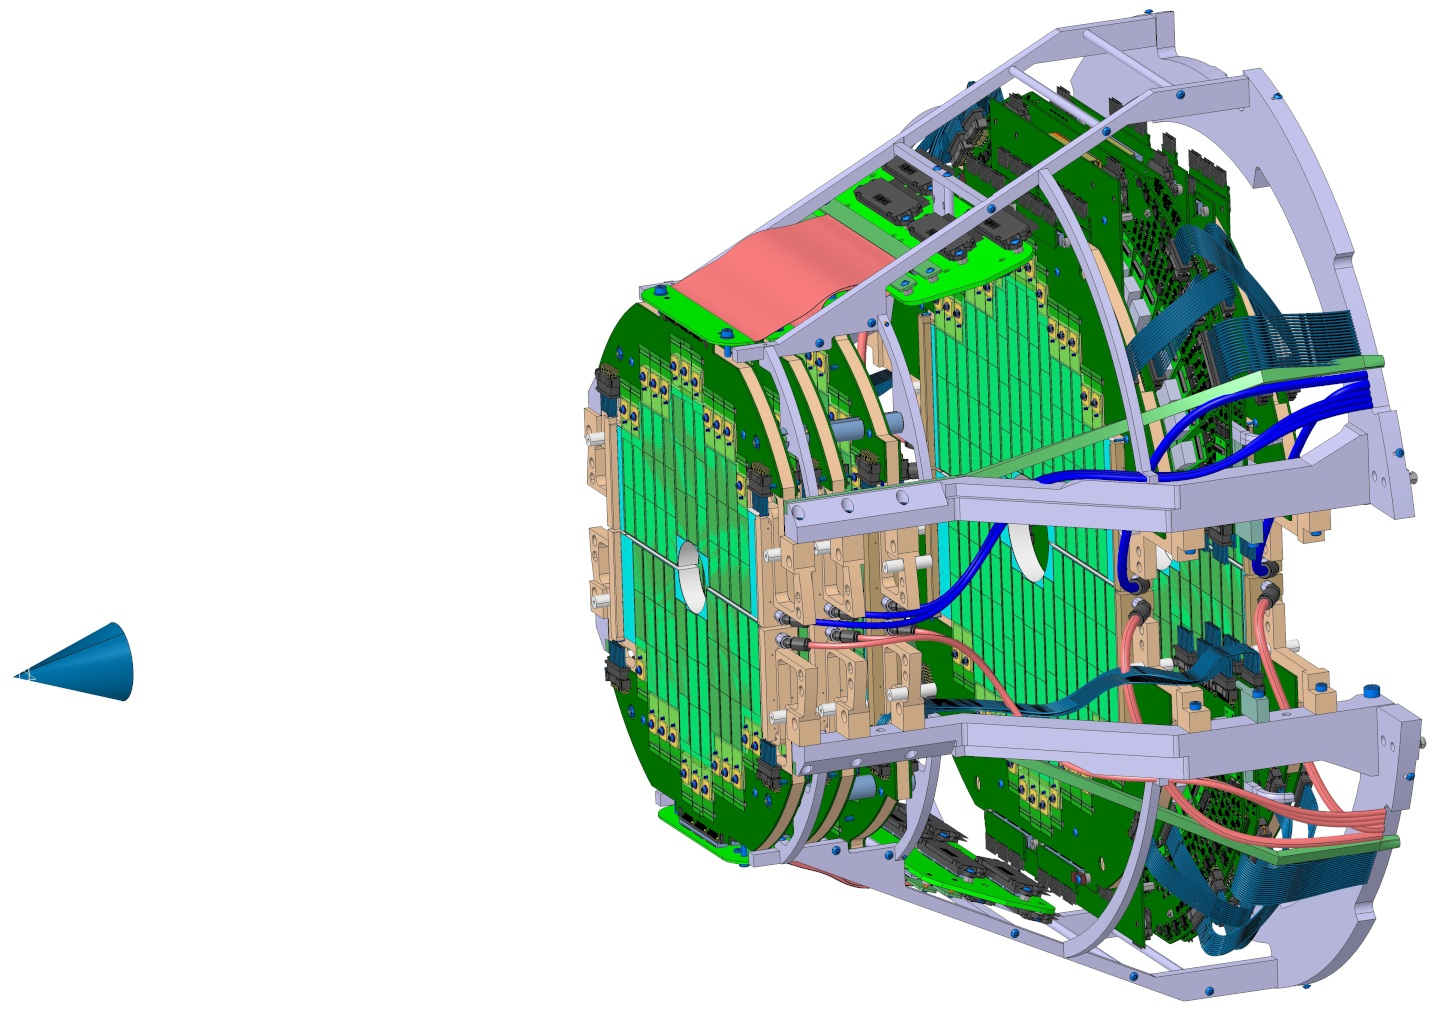
\includegraphics[keepaspectratio, scale=0.17]{fig/2_3_MFT.jpg}
                \caption{MFT}
                \label{MFT}
            \end{figure}
            The MUON spectrometer is shown in Figure \ref{MFT}\cite{MFT_TDR}. The MFT is a newly installed silicon pixel detector between $z=-46.0$ and $z=-76.8$ cm with an acceptance range of $-3.6 < \eta < -2.5$ in Run 3. It consists of 5 layers of disks that detect tracks and reconstruct MFT standalone tracks considering the influence of the L3 magnet, which creates the ALICE central magnetic field. Since the detector is placed in front of the Front Absorber, the tracks measured include muons and various other particles such as $\pi$ mesons and $K$ mesons. Combining these tracks with those measured by the backward MUON spectrometer makes it possible to measure the $DCA$ of the muons. The ability to measure $DCA$ enables the separation of muons from $c$ and $b$ quarks based on differences in lifetime. Additionally, the precision of the opening angle of the muon pair is improved, which enhances mass resolution. Furthermore, since the MFT is placed in front of the Front Absorber, it allows for the measurement of lower transverse momentum muons compared to those measured by the MUON spectrometer alone.

        \subsubsection{MFT-MUON Track Matching}\label{MFT-MUON_matching}
            The Global Track was reconstructed using the MCH Track measured with the MUON spectrometer and the MFT Track measured with the MFT. First, the MCH Tracks measured by the MUON spectrometer are extrapolated toward the collision point up to the last disk of the MFT, located at $z=76.8$ cm. The extrapolation accounts for multiple scattering and energy loss corrections in the Front Absorber between the MUON spectrometer and MFT.\@ Then, suitable MFT tracks are selected based on both position and direction, and the matching quality is evaluated by comparing the position and slope of the tracks. The best quality MFT track is selected and used to construct the Global Track.
            %begin{figure}[htbp]
            %    \centering
            %    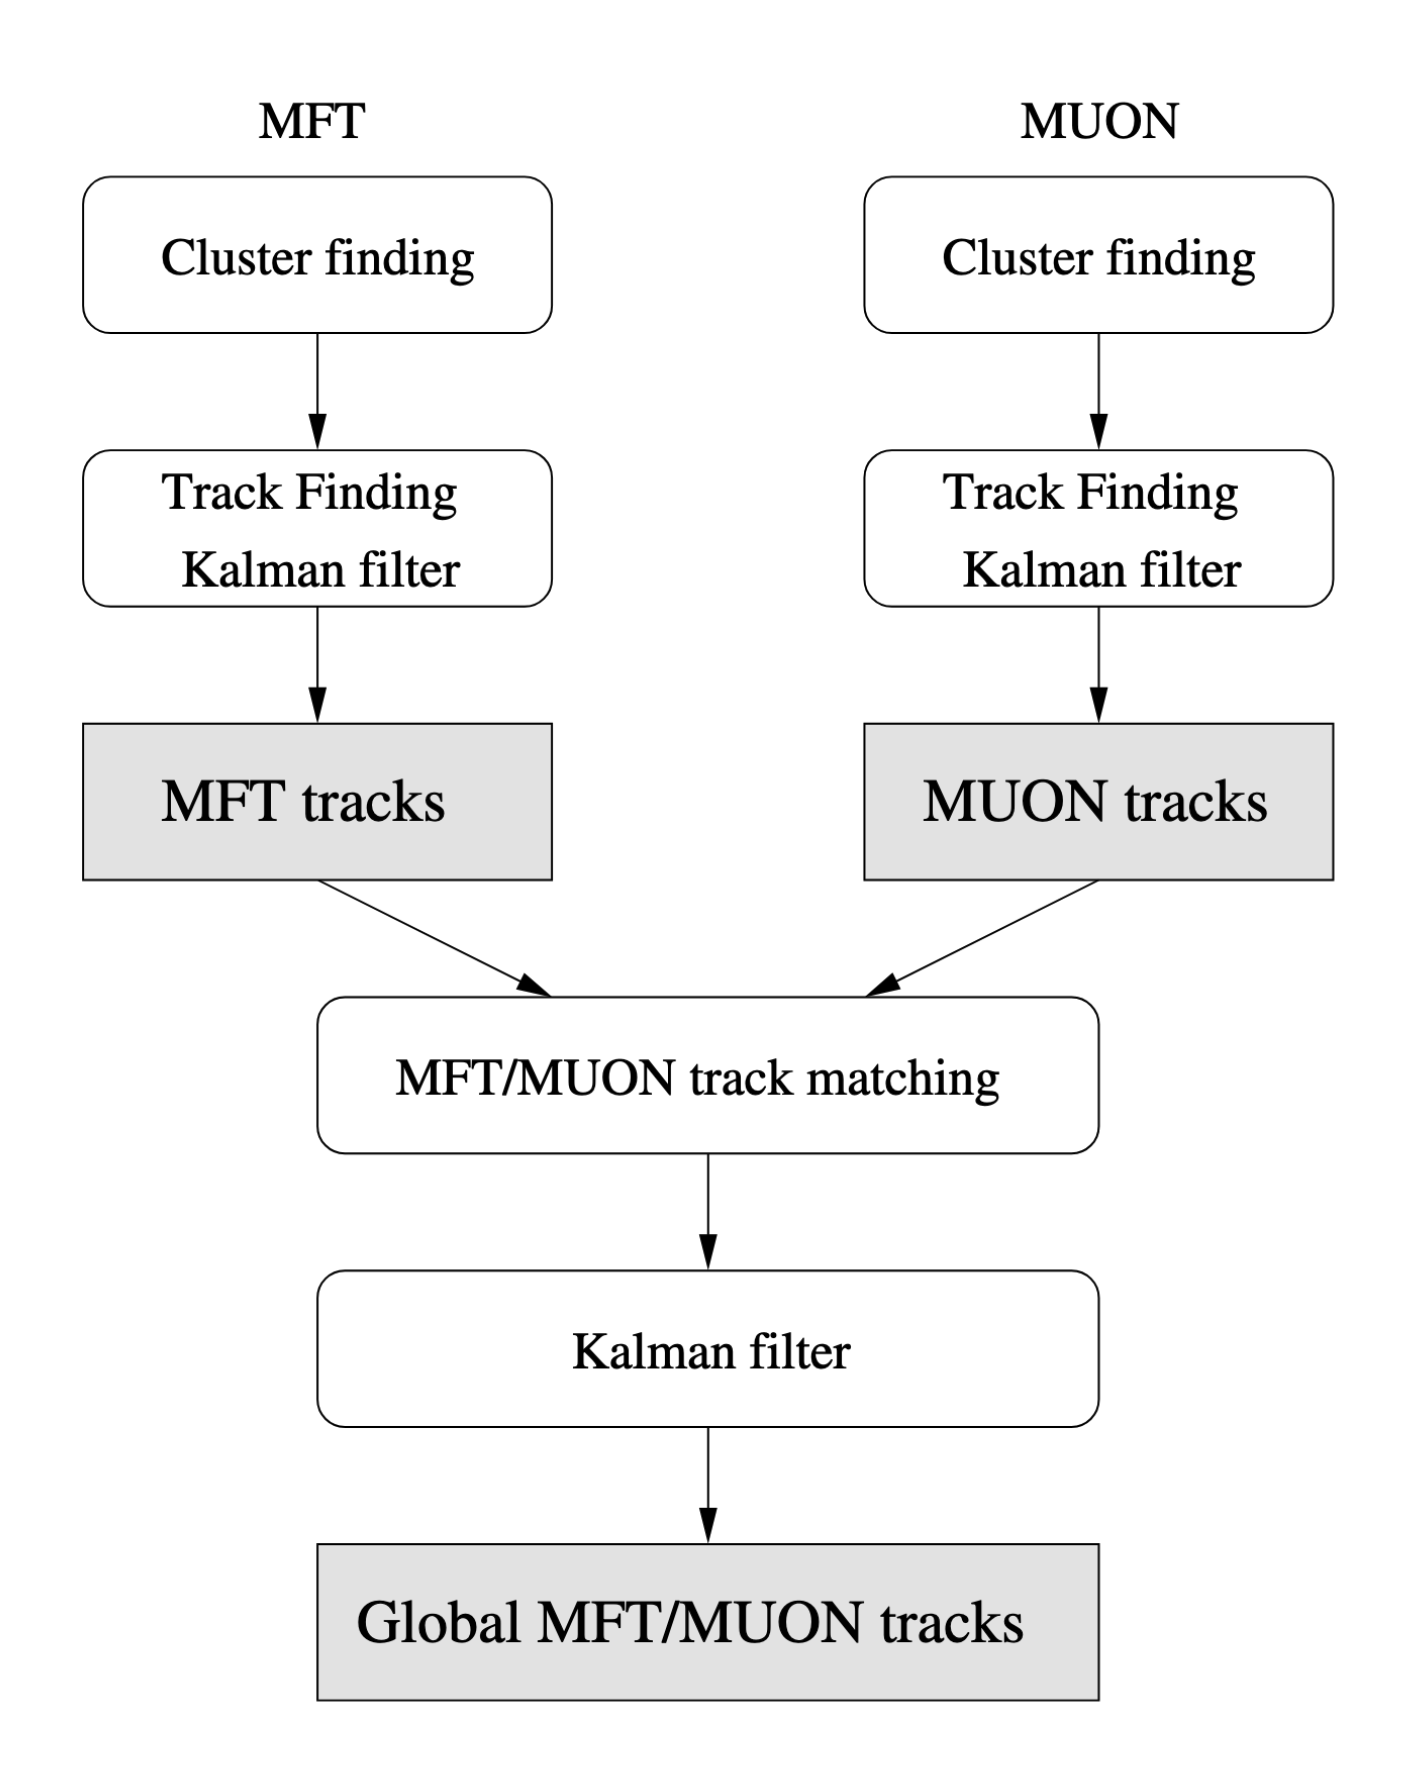
\includegraphics[keepaspectratio, scale=0.3]{fig/2_2_3_GlobalTrackReco.png}
            %    \caption{Global Track\cite{MFT_TDR}}
             %   \label{GlobalTrackReco}
            %\end{figure}
            %MUON spectrometerで測定したMCH TrackとMFTでで測定したMFT Trackを用いてGlobal Trackを再構成した。